\documentclass[11pt, letterpaper]{article}

\usepackage[bb=boondox, frak=euler]{mathalfa}
\usepackage[toc, page]{appendix}
\usepackage{amsmath}
\usepackage{braket}
\usepackage{bm}
\usepackage[colorinlistoftodos,prependcaption,textsize=tiny]{todonotes}
\usepackage{hyperref}
\usepackage{graphicx}


\author{Thomas Alexander, Zachary Schoenfeld}

\title{Project: Optimal Control Theory with Qiskit Pulse}

% Full command definitions
% Define the creation and annihilation operators for a cavity
\newcommand{\cavityCreationOperator}{a^{\dagger}}
\newcommand{\cavityAnnihilationOperator}{a}
\newcommand{\cavityNumberOperator}{\cavityCreationOperator \cavityAnnihilationOperator}
\newcommand{\iden}{\hat{\mathbb{1}}}
\newcommand{\CCCOp}{\bm{\cavityCreationOperator}}
\newcommand{\CCAOp}{\bm{\cavityAnnihilationOperator}}
\newcommand{\CCNOp}{\bm{n}}
\newcommand{\CCIOp}{\bm{\iden}}
\newcommand{\cavityOneCreationOperator}{a_1^{\dagger}}
\newcommand{\cavityOneAnnihilationOperator}{a_1}
\newcommand{\cavityOneNumberOperator}{\cavityOneCreationOperator \cavityOneAnnihilationOperator}
\newcommand{\E}[1]{\left<#1\right>}
\newcommand{\effZero}{\ket{0}}
\newcommand{\effOne}{\ket{1}}
\newcommand{\Zeff}{\sigma_z^{eff}}
\newcommand{\Xeff}{\sigma_x^{eff}}
\newcommand{\Yeff}{\sigma_y^{eff}}
\newcommand{\cavityTwoCreationOperator}{a_2^{\dagger}}
\newcommand{\cavityTwoAnnihilationOperator}{a_2}
\newcommand{\Ham}{\mathcal{H}}
\newcommand{\cavityTwoNumberOperator}{\cavityTwoCreationOperator \cavityTwoAnnihilationOperator}
\newcommand{\commutator}[2]{\left[ #1, #2 \right]}
\newcommand{\ca}{a}
\newcommand{\cc}{a^{\dagger}}
\newcommand{\cn}{n}

\newcommand{\CavityExchange}{ \left( \cavityOneCreationOperator \cavityTwoAnnihilationOperator +
    \cavityOneAnnihilationOperator \cavityTwoCreationOperator \right) }

\newcommand{\CavityCavityExchange}{\CavityExchange}

\newcommand{\cavityOneSpinExchange}{(
    \sigma^a_+ \cavityOneAnnihilationOperator +
    \sigma^a_- \cavityOneCreationOperator
    )
}
\newcommand{\cavityOneSpinExchangeSym}{(
    \sigma^a_+ \cavityOneAnnihilationOperator +
    \sigma^a_- \cavityOneCreationOperator
    )
}

\newcommand{\cavityOneSpinExchangeAntiSym}{(
    \sigma^a_+ \cavityOneAnnihilationOperator -
    \sigma^a_- \cavityOneCreationOperator
    )
}


\newcommand{\cavityTwoSpinExchange}{(
    \sigma^a_+ \cavityTwoAnnihilationOperator +
    \sigma^a_- \cavityTwoCreationOperator
    )
}

\newcommand{\cavityTwoSpinExchangeSym}{(
    \sigma^a_+ \cavityTwoAnnihilationOperator +
    \sigma^a_- \cavityTwoCreationOperator
    )
}
\newcommand{\cavityTwoSpinExchangeAntiSym}{(
    \sigma^a_+ \cavityTwoAnnihilationOperator -
    \sigma^a_- \cavityTwoCreationOperator
    )
}

% Shortened command definitions
\newcommand{\com}[2]{\commutator{#1}{#2}}
\newcommand{\cavA}{\cavityAnnihilationOperator}
\newcommand{\cavC}{\cavityCreationOperator}
\newcommand{\cavN}{\cavityNumberOperator}

\newcommand{\cavAOne}{\cavityOneAnnihilationOperator}
\newcommand{\cavCOne}{\cavityOneCreationOperator}
\newcommand{\cavNOne}{\cavityOneNumberOperator}

\newcommand{\cavATwo}{\cavityTwoAnnihilationOperator}
\newcommand{\cavCTwo}{\cavityTwoCreationOperator}
\newcommand{\cavNTwo}{\cavityTwoNumberOperator}


\DeclareMathOperator{\Tr}{Tr}
\DeclareMathOperator*{\argmax}{arg\,max}
\DeclareMathOperator*{\argmin}{arg\,min}


\begin{document}
\maketitle
\tableofcontents

\section{Introduction}
Optimal control theory studies how to optimally (given an objective) manipulate a quantum system
to guide a state through a desired evolution given available classical
stimulus sources. Qiskit Pulse exposes control of quantum computing
stimulus sources through a standardized API, making lab-level experiments
possible through the cloud. In Qiskit a quantum circuit is lowered to a pulse
schedule through a scheduling procedure using predefined gate to pulse schedule
calibrations.

The aim of this project is to explore incorporating optimal control theory
into the Qiskit compilation pipeline with the aim of enabling on the fly
gate design of arbitrary unitary evolutions for applications in Qiskit Aqua.
Specifically you will examine implementing GRAPE \cite{khanejaOptimalControlCoupled2005c} on
a single-qubit IBM Quantum device.
This idea was explored in the work of Shi et. al. \cite{shiOptimizedCompilationAggregated2019b}
(see Figure \ref{fig:compilationpipeline}) with their focus on dynamic gate
aggregation and design.

\begin{figure}[hbt!]
 \centering
 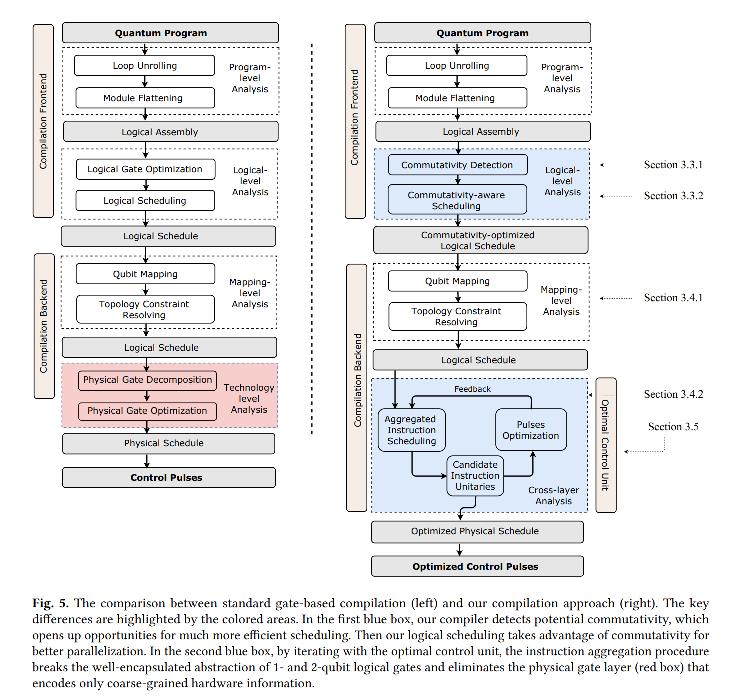
\includegraphics[width=\linewidth]{../figures/yunong_pipeline.png}
 \caption{Compilation pipeline proposed by Shi et. al., reproduced from \cite{shiOptimizedCompilationAggregated2019b}.}
 \label{fig:compilationpipeline}
\end{figure}

We will begin to build out this functionality into Qiskit.
You will take the first exploratory steps of performing optimal control on actual qubits with Qiskit
Pulse and then come up with a proposal for how to add this functionality
to the Qiskit compilation pipeline in production.

\subsection{Overall Goals}
\begin{itemize}
\item Design and implement an optimal pulse control pipeline for constructing single qubit quantum gates
\item Develop your physics and software skills by applying them to optimal control theory
\item Gain exposure to the agile development processes and working with a full stack team across software and hardware
\item Have some fun!
\end{itemize}


\subsubsection{Technical Goals}
\begin{itemize}
\item Understand in a broad sense the engineering of superconducting qubits \cite{blaisCavityQuantumElectrodynamics2004c, krantzQuantumEngineerGuide2019a}.
\item Bootstrap control of a qubit with Qiskit Pulse. See \cite{CalibratingQubitsQiskit}.
\item Model the Hamiltonian of your system and simulate it.
\item Understand the goal of optimal control and how GRAPE works \cite{khanejaOptimalControlCoupled2005c}.
\item Select a Python GRAPE package for incorporation into Qiskit. Examples include \cite{QuantumOptimalControl, SchusterLabQuantumoptimalcontrol2020, abdelhafezGradientbasedOptimalControl2019, QuantumUtilsMathematica}.
\item Estimate the Hamiltonian of a single qubit with Qiskit Pulse \cite{alexanderNotebooksDataQiskitPulse2020b, hincksHamiltonianLearningOnline2018, sheldonProcedureSystematicallyTuning2016b}.
\item Design arbitrary single qubit gates with Grape and Qiskit Pulse and characterize the gates with quantum process tomography \cite{alexanderNotebooksDataQiskitPulse2020b}.
\item Hack automated gate design into the Qiskit compilation pipeline.
\item Write a report reviewing the relevant underlying theory, your methodology and findings performing optimal control theory with Qiskit pulse.
Include a design section proposing how to implement automated gate aggregation \cite{shiOptimizedCompilationAggregated2019b} and compilation within Qiskit and any improvements that might be required.
\item Stretch goals (in no particular order other than what would be most fun for me)

\begin{itemize}
\item Estimate the Hamiltonian for a two-qubit system and design a two-qubit gate with Qiskit Pulse and GRAPE.
\item Reduce the runtime of an Aqua application with automated gate design.
\item Design a gate aggregation pass in the Qiskit transpiler to work with your pulse designer.
\item Suggest how to improve the usability of the Qiskit Pulse simulator.
\end{itemize}
\end{itemize}

\subsection{Workflow}
Due to the nature of the situation with Covid-19 the internship will be remote.
Fortunately, this project is focused on Qiskit Pulse, which gives hardware access
through the cloud. To help facilitate work both Thomas Alexander and
Zachary Schoenfeld will be providing supervision. Ben will partcipate in the
pulse teams agile sprints, demos and board. We will hold short, daily video
calls to synchronize our work. There will also be many other remote activities
setup for interns to network and socialize through the IBM Quantum Internship
program.\\
%
\\
%
IBM Quantum intern hub: \url{https://w3.ibm.com/w3publisher/quantum-interns}.

\subsection{Approximate Timeline (Subject to Change)}

Dates: 6/5/20-8/7/20 (8 weeks) \\
\\
%
Weeks 1, 2
\begin{itemize}
\item Onboard
	\begin{itemize}
		\item Get onto w3, Slack, join standups and agile
	\end{itemize}
\item Gain familiarity with IBM's quantum systems and pulse-level control (ask for more papers!)
\item Use Qiskit pulse to calibrate a qubit on a live device
\item \textit{Suggestion}: Draft notes as you go. This will make writing the final report easier!
\end{itemize}
Weeks 3, 4
\begin{itemize}
\item Model a 1q Hamiltonian with arbitrary drive pulse and simulate its evolution
	\begin{itemize}
		\item It may also be interesting to learn how to analytically solve this Hamiltonian for simple pulses shapes (RWA, etc)
	\end{itemize}
\item Learn GRAPE and explore possible open source packages for implementation into Qiskit
\end{itemize}
Weeks 5, 6
\begin{itemize}
\item Use chosen GRAPE package and Qiskit pulse to construct arbitrary 1q gates in an optimal fashion
\item Characterize these gates with Quantum Process Tomography
\item Begin to integrate GRAPE into the Qiskit compilation pipeline
\end{itemize}
Weeks 7, 8
\begin{itemize}
\item As time permits, think about how to add gate aggregation passes \cite{shiOptimizedCompilationAggregated2019b} to your work (design is more important; can implement if time)
\item Write up a report detailing the theory you learned about optimal pulse control, GRAPE and how you implemented it in Qiskit. More details provided in the \textbf{Goals} section.
\item As time permits, work on the stretch goals outlined in the \textbf{Goals} section
\item Offboard
\end{itemize}



\bibliographystyle{unsrt}
\bibliography{bibliography}

\end{document}
